% !TEX root = ../Report.tex
\subsection{DeepMedic architecture}
DeepMedic is a 3D neural network. It has been initially used for segmentations in biomedical 3D scans, especially for detecting brain anomalies such as injuries, tumors and lesions. In this project we will try this algorithm for lung segmentations. \newline 
A DeepMedic model consists of detecting a particular pattern in an image. This is achieved by multi-layer convolution in the network. We distinguish two components in the model. First there is a three-dimension convolutional neural network (CNN) model used for dense segmentation, then  a three-dimension fully connected conditional random field (CRF) model for deeper predictions. (Might we only use the first component?) \newline
Each layer of the CNN model contains channels called feature maps, i.e. a group of neurons identifying a feature in the previous layer. Then a feature is defined by associated kernel weights. Number of inputs, outputs, feature-maps and kernels are tunable.

\begin{figure}[h!]
	\includegraphics[width=0.49\textwidth, angle=0]{files/deepmedic.png}
	\caption{ Overview of DeepMedic architecture}
	\label{deepmedic}
\end{figure}

\subsection{U-Net architecture}
Semantic segmentation is partition of an image in coherent parts. U-Net is mostly used for biomedical image segmentation. In figure \ref{unetstructure} the structure of the U-Net is shown.\newline

\begin{figure}[h!]
	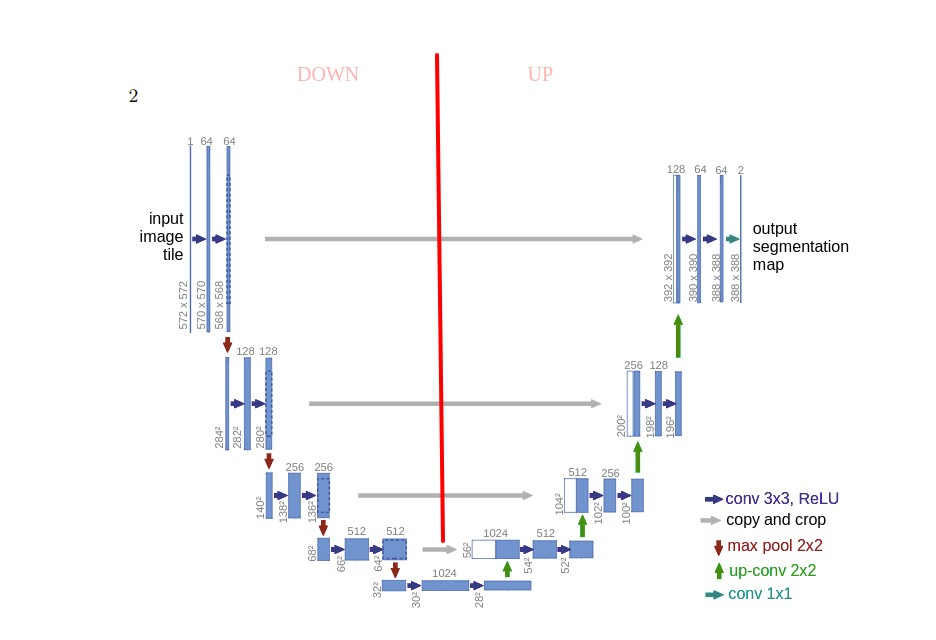
\includegraphics[width=0.49\textwidth, angle=0]{files/unetstructure.jpg}
	\caption{Structure of U-Net architecture}
	\label{unetstructure}
\end{figure}

Each blue box corresponds to a multi-channel feature map. The number of channels is denoted on top of the box. X-Y-size is provided at the lower left edge. White boxes represent copied feature maps. Arrows denote the different operations.\newline
First part is called down or encoder part. Convolutional blocks followed by maxpool downsampling layers are applied to encode the input image into feature representations at multiple different levels. The second part of the network consists of upsampling and concatenation layers followed by regular convolution operations. The dimensions from left are expanded to meet the original image size. The grey and green arrows indicate where to concatenate future maps together.\newline
In comparison to other fully convolutional segmentation networks, the main feature of U-Net  is that while upsampling and going deeper in the networks, it also concatenates the higher resolution features from the down sampling part with upsampled features in order to better localize and learn representation.\newline
%As upsampling is sparse we need to be good prior from beginning stages to get the better localization representation. In order to get consistent size, we applied padded convolutions to keep dimensions across concatenation. Localization is one of the most important features in case of biomedical image processing. In order to localize, high resolution from the contracting path are combined with upsampled output. By this the successive convolution layer can then learn to assemble a more precise output. The main modification in our architecture was that in the upsampling part we have a large number of feature channels, which allows the network to propogate context information to high resolution layers. To predict the pixels in the border region of the image, the missing context is extrapolated by mirroring the input image.

\subsection{Metrics}

\subsubsection{Dice Loss}
formulas
\subsubsection{BCE Dice Loss}

\subsubsection{Hausdorff distance}

\subsubsection{Mean distance}